\documentclass[11pt,a4paper]{article}
\usepackage[utf8]{inputenc}
\usepackage[croatian]{babel}
\usepackage{amsmath, amsfonts, amssymb}
\usepackage{tocloft}
\usepackage[hidelinks]{hyperref}
\usepackage[section]{placeins}
\usepackage{graphicx}
\usepackage{float}
\bibliographystyle{ieeetr}%ieeetr, abbrv
\renewcommand{\cftsecleader}{\cftdotfill{\cftdotsep}}



\newcommand{\kolegij}{Elementi strojeva 2}
\newcommand{\naslovRada}{Projektni zadatak}
\newcommand{\mailFriendlynaslovRada}{Elementi strojeva 2, projektni zadatak}

\author{Kristijan Cetina\footnote{\href{mailto:kcetina@politehnika-pula.hr?subject=\mailFriendlynaslovRada}{kcetina@politehnika-pula.hr}, JMBAG: 2424011721}}
\title{\kolegij \\ \naslovRada}
\date{Pula, \today}

\begin{document}

\begin{titlepage}
\clearpage
\begin{center}
\begin{Huge}
POLITEHNIKA PULA\\
\end{Huge}
\begin{LARGE}
Visoka tehničko-poslovna škola s p.j.\\
Stručni studij politehnike\\
\end{LARGE}
\end{center}
\vspace{3cm}
{\let\newpage\relax\maketitle}
\thispagestyle{empty}
\vfill
\begin{abstract}
U ovom radu predstavljam proračun strojnog sklopa - vratila prijenosnika snage i pripadajućih ležajeva koji je zadan kao sastavni dio kolegija Elementi strojeva 2.
\end{abstract}
\end{titlepage}

\tableofcontents
%\listoftables	%ako ih ima puno prebaci na kraj dokumenta
%\listoffigures	%ako ih ima puno prebaci na kraj dokumenta

\newpage
\section{Uvod}
Ovaj projektni zadatak nastoj je kao obavezni zadatak u sklopu kolegija Elementri strojeva 2 koji se održava pod vodstvom prof. dr. sc. Božidara Križana na stručnom studiju politehnike na Politehnici Pula.

U ovom radu obrađen je proračun vratila prijenosnika snage s pripadajućim ležajevima. Prema zadatku bilo je potrebno odrediti dimenzije vratila i ležaja te odabrati prikladni ležaj u ondnosu na postavljene zahtjeve prenosa snage i traženu minimalnu trajnost.

\newpage
\section{Proračun sklopa}
\subsection{Zadani parametri}
Prema projektnom zadatku zadani su sljedeći parametri sklopa:\\
Snaga koju prenose zučanik i vratilo
\begin{tabbing}
\hspace{260pt}\=\kill
 Snaga koju prenose zupčanik i vratilo \> $P=23 kW$ \\ 
 Brzina vrtnje \> $800 min^{-1}$ \\ 
 Materijal vratila \> Ck45 \\
 Korjeni promjer zupčanika \> $d_f=96,25mm$ \\ 
 Diobeni promjer zupčanika \> $d=110mm$ \\ 
 Tjemeni promjer zupčanika \> $d_a=121mm$ \\ 
 Širina zupčanika \> $b_z=115mm$ \\ 
 Faktor sigurnosti \> $\nu_d=1,3$ \\ 
 Hrapavost površine na kritičnim mjestima \> $R_a=0,8\mu m$ \\ 
 Razmak ležajeva \> $l=165mm$ \\ 
 Razmak između središta ležaja A\\ i središta zupčanika \> $a=80mm$ \\ 
 Minimalna trajnost ležajeva \> $L_{10h min}=12000 sati$
\end{tabbing}
Mehanička svojstva korištenog materijala su sljedeća:\\
\begin{align*}
R_{dt0}&=340 \textstyle\frac{N}{mm^2}\\
R_{ds-1}&=370 \textstyle\frac{N}{mm^2}\\
R_e&=490 \textstyle\frac{N}{mm^2}\\
R_m&=700 \textstyle\frac{N}{mm^2}
\end{align*}
 
\subsection{Projektni proračun sklopa}
U projektnom praračunu sklopa ne uzima se u obzir svi detalji sklopa kao niti koncentracije lokalnog naprezanja, ali se zato uzima značajno veći faktor sigurnosti kako bi kompenzirali za izostavljene faktore. U projektnom proračunu za određivanje početnog promjera vratila uzeti su u obzir samo snaga koja se prenosi i materijal od kojeg se izrađuje vratilo. Kao mjerodavne vrijednosti uzeto je torzijsko naprezanje koje mora biti manje od dopuštenog, a faktor sigurnosti je usvojen $\nu=12$.
Kao glavni uvjet uzet je kriterij čvrstoće pri kojem torzijsko naprezanje mora biti manje od dopuštenog pri čemu torzijsko naprezanje možemo izraziti pomoću izraza
\begin{equation}
\tau_t=\dfrac{T}{W_p}\label{equ:tangencijalnoNaprezanje}
\end{equation}
pri čemu je $W_p$ za okrugli puni popreči presjek jednak
\begin{equation}
W_p=\frac{d_1^3 \cdot \pi}{16}
\end{equation}
Okretni moment koji se prenosi izračunat je pomoću sljedećeg izraza
\begin{equation}
T=\frac{P}{\omega}\label{equ:okretniMoment}
\end{equation}
pri čemu je obodna brzina $\omega=2 \cdot \pi \cdot n$, a $n$ je izražen u okretajima u sekundi $[s^{-1}]$.
Uvršavanjem poznatih podataka u \eqref{equ:okretniMoment} dobije se okretni moment
\begin{align*}
T&=\frac{60 \cdot 23 \cdot 10^3}{2 \cdot \pi \cdot 800}\\
T&=\textbf{274,5 Nm}
\end{align*}
Promjer vratila je izračunat pomoću izraza
\begin{equation}
d_1 \geq \sqrt[3]{\dfrac{16 \cdot T \cdot \nu}{R_{dt0} \cdot \pi}} \label{equ:pocetniPromjer}
\end{equation}

Uvršavanjem poznatih podataka u izraz \eqref{equ:pocetniPromjer} dobije se početni promjer vratila $d_1$
\begin{align*}
d_1&\geq \sqrt[3]{\dfrac{16 \cdot 274,5\cdot 10^3 \cdot 12}{340 \cdot \pi}}\\
d_1&\geq \mathbf{36,68 mm} 
\end{align*}

\subsection{Konstruiranje sklopa}
Prema tablici standardnih dimenzija krajeva cilindričnog vratila prema normi DIN 748 usvojena je dimenzija \textbf{38x80 DIN 748} ($\phi38k6$). Maksimalni radijus prijelaza je $r_{max}=1 mm$.

Prema tablici standardnih dimenzija uložnih pera po DIN 6885 normi usvojeno je pero 
$\mathbf{DIN6885-A 10 \times 8 \times 70-E295}$ s dubinom utora u vratilu $t_1=5mm$.
Dimenzija $d_2$ je zbog standardnih dimenzija ležajeva usvojena $\mathbf{d_2=45mm}$
\subsubsection*{Žlijeb za izlaz alata}
Usvojeme dimenzije žlijeba za izlaz alata prema $d_2$ su $\mathbf{DIN \, 509-E \, 0,6 \times 0,3}$ ($\rho_1=0,6mm$, $t_1=0,3mm$). Na slici \ref{izlazAlata} prikazan je žlijeb za izlaz alata.
\begin{figure}[H]
\centering
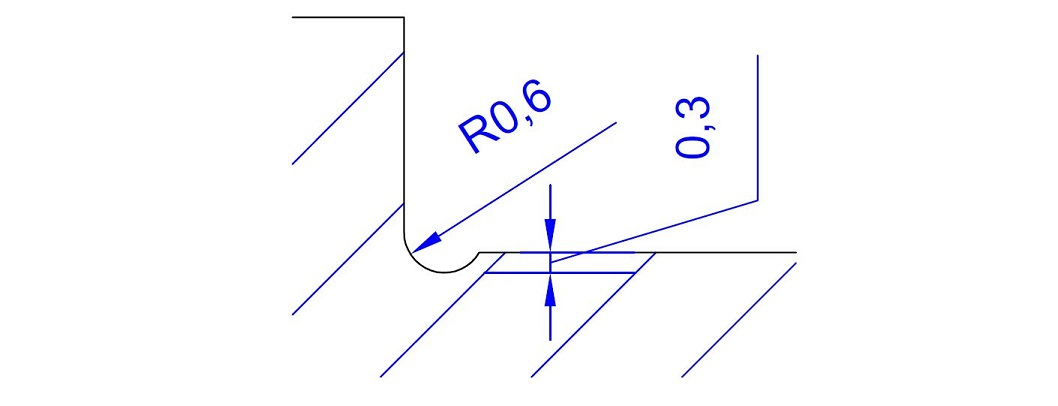
\includegraphics[width=1\textwidth]{izlazAlata}
\caption{Skica žlijeba za izlaz alata}\label{izlazAlata}
\end{figure}
\subsubsection*{Visina bočnog oslonca ležaja}
Kao vrijednost visine bočnog oslonca ležaja usvojena je vrijednost $h=3,5mm$.
Promjer $d_3$ je izračunat kao $d_3=d_2+2 \cdot h = \mathbf{52mm}$.
Vrijednost radijusa zakrivljenja $\rho_2$ je usvojen $\rho_2=5mm$.

\subsection{Proračun reakcija u ležajevima}
Tangencijalna sila između zupčanika je izračunata pomoću momenta koji se prenosi i promjera zupčanika
\begin{align*}
F_t&=\frac{2T}{d}\\
F_t&=\frac{2 \cdot 274,5 \cdot 10^3}{110}\\
F_t&=\textbf{4990,9N}
\end{align*}
Radijalna sila je izračunata pomoću tangencijalne sile i poznatog kuta zahvata zubaca zupčanika koji iznosi $\alpha_n=20^\circ$
\begin{align*}
F_r&=F_t \cdot \tan \alpha_n\\
F_r&=4990,9 \cdot \tan 20^\circ\\
F_r&=\textbf{1816,5N}
\end{align*}
Kako sile mođusobno djeluju pod pravim kutem njihova rezultanta se može izračunati po Pitagorinom poučku kao korijen zbroja kvadrata sila
\begin{align*}
F&=\sqrt{F_t^2 + F_r^2}\\
F&=\sqrt{4990,9^2 + 1816,5^2}\\
F&=\textbf{5311,2N}
\end{align*}
Reakcija u osloncu $B$ izračunata je pomoću uvijeta ravnoteže sume momenata oko oslonva $A$
\begin{align*}
F_B&=\frac{F \cdot 80}{168}\\
F_B&=\frac{5311,2N \cdot 80}{168}\\
F_B&=\textbf{2575,1N}
\end{align*}
rakcija u osloncu $A$ izračunata je pomoću uvijeta ravnoteže sustava u kojem je suma sila i reakcija jednaka nuli
\begin{align*}
F_A&=F-F_B\\
F_A&=5311,2-2575,1\\
F_A&=\textbf{2736,1N}
\end{align*}

\subsection{Izbor valjnih ležajeva i proračun stvarne trajnosti}
Trajnost ležajeva se može proračunati po izrazu
\begin{equation}
L_{10h}=\left(\frac{C}{F} \cdot f_t \right)^p \cdot \frac{10^6}{60 \cdot n}
\label{equ:trajnostLezaja}
\end{equation}
pri čemu je $C$ - dinamička nosivost ležaja, $p$ - eksponent vijeka trajanja. Za kuglične ležajeve $p=3$ i $f_t$ - temperaturni faktor. Za $\vartheta < 150^\circ C \Rightarrow f_t=1$.

Iz izraza \eqref{equ:trajnostLezaja} može se izračunati minimalna potrebna dimanička nosivost ležaja
\begin{align*}
C&=\frac{F}{f_t} \cdot \sqrt[3]{\frac{L_{10h} \cdot 60 \cdot n}{10^6}}\\
C&=\frac{2736,1}{1} \cdot \sqrt[3]{\frac{12000 \cdot 60 \cdot 800}{10^6}}\\
C&\cong \mathbf{22,8kN}
\end{align*}
Nakon pregleda kataloških podataka dostupnih ležajeva odabran je ležaj \textbf{SKF 6209} koji ima dinamičku nosivost od $C=35,1kN$.

\begin{figure}[!h]
\centering
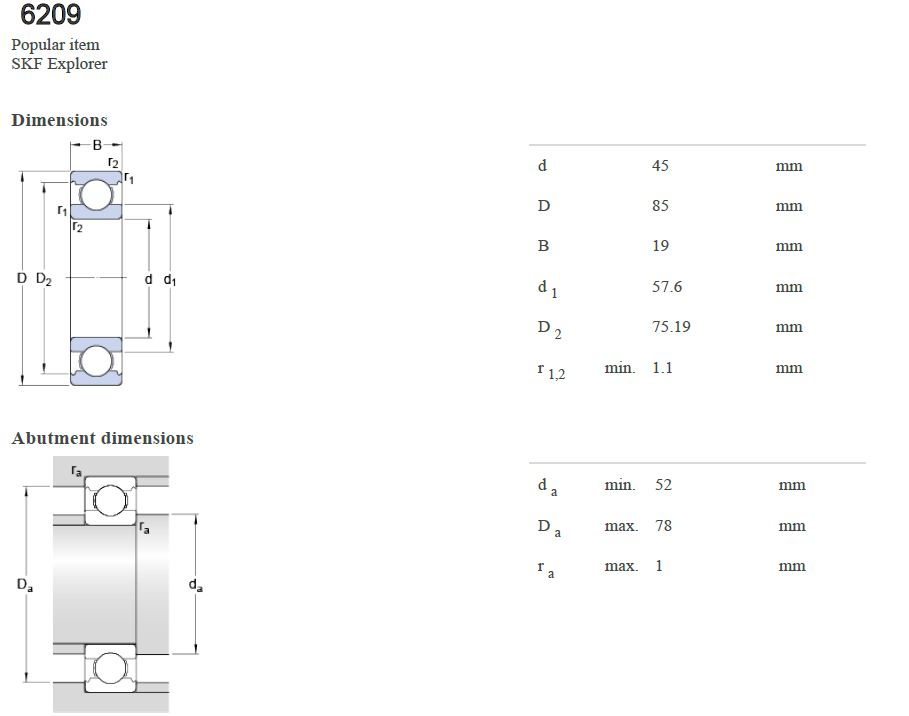
\includegraphics[width=1\textwidth]{6209_data}
\caption{Tehnički podaci odabranog ležaja SKF 6209}\label{6208data}
\end{figure}

\subsubsection*{Proračun stvarne trajnosti}
Po izrazu \eqref{equ:trajnostLezaja} sada se može izračunati stvarna trajnost za odabrani ležaj
\begin{align*}
L_{10h}&=\left(\frac{35100}{2736,1} \cdot 1 \right)^3 \cdot \frac{10^6}{60 \cdot 800}\\
L_{10h}&=\mathbf{43983\, h}
\end{align*}

\newpage

\subsection{Proračun momenata savijanja i naprezanja}
U nastavku su dani proračuni momenata savijanja i naprezanja za svaki kritični presjek nazanačen na slici \ref{KriticniPresjeci}.
\begin{figure}[h]
\centering
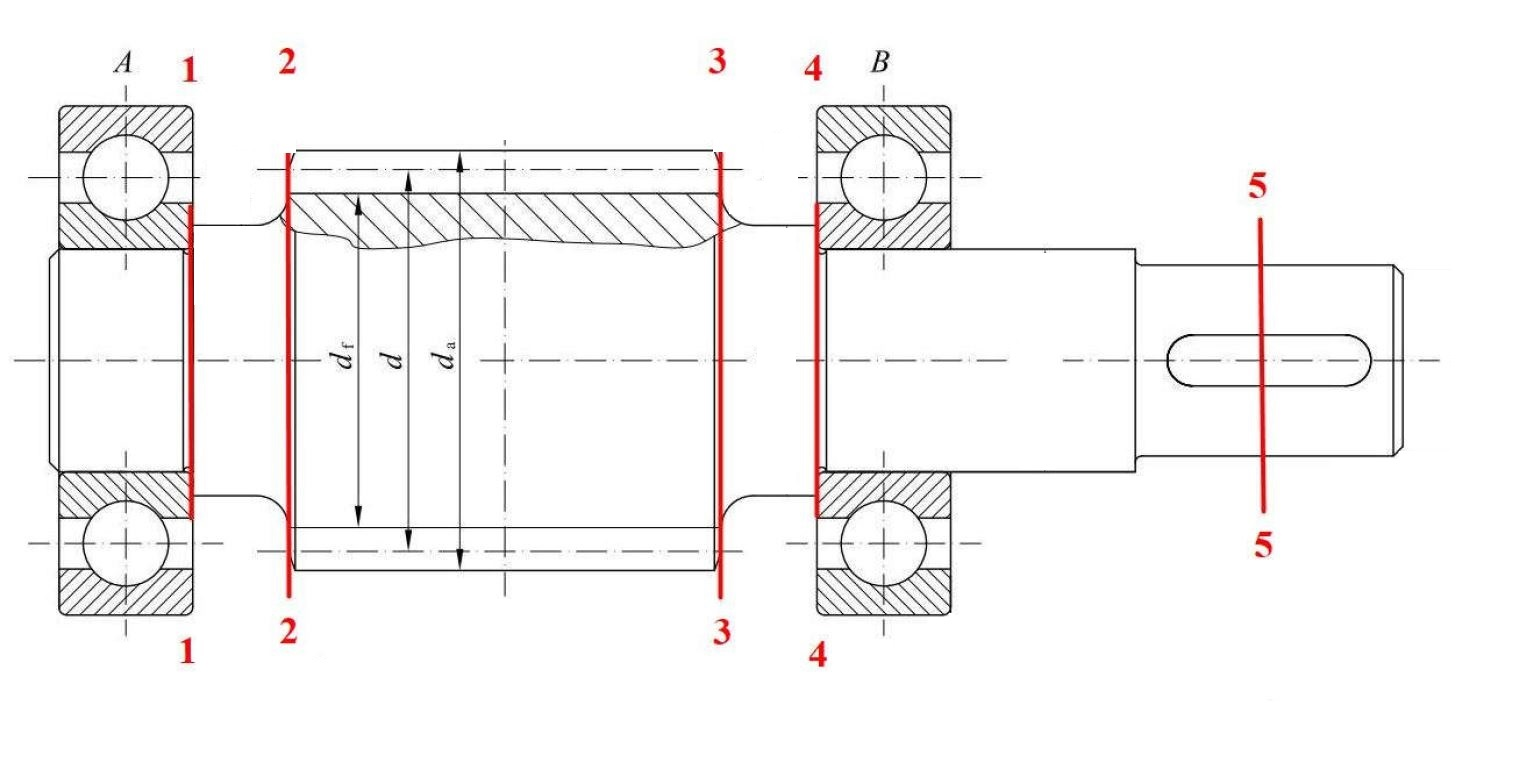
\includegraphics[width=1\textwidth]{KriticniPresjeci}
\caption{Prikaz kritičnih presjeka na vratilu}\label{KriticniPresjeci}
\end{figure}
\begin{align*}
M_{S1}=F_A \cdot \frac{B}{2}=2736,1 \cdot \frac{19}{2}&=25933Nmm\\
M_{S2}=F_A \cdot \left(a- \frac{b_z}{2}\right)=2736,1 \cdot \left(80- \frac{115}{2}\right)&=61562,3Nmm\\
M_{S3}=F_B \cdot \left(l-a- \frac{b_z}{2}\right)=2575,1 \cdot \left(165-80- \frac{115}{2}\right)&=70815,3Nmm\\
M_{S4}=F_B \cdot \frac{B}{2}=2575,1 \cdot \frac{19}{2}&=24463,5Nmm\\
M_{S5}&=0
\end{align*}

\subsubsection*{Geometrijske karakteristike poprečnih presjeka - $W$}
\begin{align*}
W_1=W_4=\frac{d_2^3 \cdot \pi}{32}=\frac{45^3 \cdot \pi}{32}&=8946,2mm^3\\
W_2=W_3=\frac{d_3^3 \cdot \pi}{32}=\frac{52^3 \cdot \pi}{32}&=13804,2mm^3
\end{align*}
\subsubsection*{Polarni momenti otpora - $W_p$}
\begin{align*}
W_{p2}=W_{p3}=\frac{d_3^3 \cdot \pi}{16}=\frac{52^3 \cdot \pi}{16}&=27608,3mm^3\\
W_{p4}=\frac{d_2^3 \cdot \pi}{16}=\frac{45^3 \cdot \pi}{16}&=17892,4mm^3\\
W_{p5}=\frac{(d_1-t_1)^3 \cdot \pi}{16}=\frac{(38-5)^3 \cdot \pi}{16}&=7056,2mm^3
\end{align*}
\subsubsection*{presjek 1-1}
$$
\sigma_{s1}=\frac{M_{S1}}{W_1}=\frac{25933}{8946,2}=\mathbf{2,9\textstyle\frac{N}{mm^2}}
$$
\subsubsection*{presjek 2-2}
\begin{align*}
\sigma_{s2}=\frac{M_{S2}}{W_2}=\frac{61562,3}{13804,2}&=4,6\textstyle\frac{N}{mm^2}\\
\tau_{t2} =\frac{T}{W_{p2}}=\frac{274,5 \cdot 10^3}{27608,3}&=9,9\textstyle\frac{N}{mm^2}\\
\sigma_{ekv2}=\sqrt{\sigma_{s2}^2+3 \cdot (0,7 \cdot \tau_{t2})^2}\\
\sigma_{ekv2}=\sqrt{4,6^2+3 \cdot (0,7 \cdot 9,9)^2}&=\mathbf{12,9\textstyle\frac{N}{mm^2}}
\end{align*}
\subsubsection*{presjek 3-3}
\begin{align*}
\sigma_{s3}=\frac{M_{S3}}{W_3}=\frac{70815,3}{13804,2}&=5,1\textstyle\frac{N}{mm^2}\\
\tau_{t3} =\frac{T}{W_{p3}}=\frac{274,5 \cdot 10^3}{27608,3}&=9,9\textstyle\frac{N}{mm^2}\\
\sigma_{ekv3}=\sqrt{\sigma_{s3}^2+3 \cdot (0,7 \cdot \tau_{t3})^2}\\
\sigma_{ekv3}=\sqrt{4,6^2+3 \cdot (0,7 \cdot 9,9)^2}&=\mathbf{13 \textstyle \frac{N}{mm^2}}
\end{align*}
\subsubsection*{presjek 4-4}
\begin{align*}
\sigma_{s4}=\frac{M_{S4}}{W_4}=\frac{23175,9}{8946,2}&=2,6\textstyle\frac{N}{mm^2}\\
\tau_{t4} =\frac{T}{W_{p4}}=\frac{274,5 \cdot 10^3}{17892,4}&=15,3\textstyle\frac{N}{mm^2}\\
\sigma_{ekv4}=\sqrt{\sigma_{s4}^2+3 \cdot (0,7 \cdot \tau_{t4})^2}\\
\sigma_{ekv4}=\sqrt{2,6^2+3 \cdot (0,7 \cdot 15,3)^2}&=\mathbf{18,7 \textstyle\frac{N}{mm^2}}
\end{align*}
\subsubsection*{presjek 5-5}
$$
\tau_{t5} =\frac{T}{W_{p5}}=\frac{274,5 \cdot 10^3}{7056,2}=\mathbf{38,9\textstyle\frac{N}{mm^2}}
$$

\section{Kontrolni proračun vratila}
Dopušteno naprezanje pri savijanju u kontrolnom proračunu uzima u obzir trajnu izmjeničnu dinamičku čvrstoću materijala pri savijanju, faktore $b_{1 \sigma}$ - faktor utjecaja poršinske hrapavosti za vlak/tlak i savijanje, $b_2$ - faktor utjecaja veličine konstrukcijskog elementa, $\nu_d$ - faktor sigurnosti prikladan za kontrolni proračun te $\beta_{ks}$ - efektivni faktor koncentracije naprezanja pri savijanju i to sve u sljedećem izrazu
\begin{equation}
\sigma_{sdop}=\frac{R_{ds-1} \cdot b_{1 \sigma} \cdot b_2}{\nu_d \cdot \beta_{ks}}\label{equ:dozvoljenoNaprezanje_kontrolni_savijanje}
\end{equation}
Za izračunati dopušteno naprezanje potrebni su i sljedeći podaci
\begin{align*}
R_z&=4 \cdot R_a\\
R_z&=4 \cdot 0,8 \mu m\\
R_z&=\mathbf{3,2 \mu m}
\end{align*}
Faktor $b_{1 \sigma}$ vrijedi isti za cijeli sklop jer je navedeni kompletan izrađen od istog materijala jednake površinske obrade, a izračunat je po sljedećem izrazu
\begin{align*}
b_{1 \sigma}&=1-0,22 \cdot \log R_z \left( \log \frac{R_m}{20}-1 \right)\\
b_{1 \sigma}&=1-0,22 \cdot \log 3,2 \left( \log \frac{700}{20}-1 \right)\\
b_{1 \sigma}&=\mathbf{0,939}
\end{align*}
Efektivni faktor koncentracije naprezanja pri savijanju $\beta_{ks}$ se računa za svaki kritični presjek i to po izrazu
\begin{equation}
\beta_{ks}=1+ \eta_k \cdot (\alpha_{ks}-1)\label{equ:beta_KS}
\end{equation}
Faktor osjetljivosti materijala na koncentraciju naprezanja $\eta_k$ se računa po sljedećem izrazu
\begin{equation}
\eta_k=\frac{1}{1+\frac{8}{\rho} \cdot \left( 1- \frac{R_e}{R_m} \right)^3}\label{equ:eta_K}
\end{equation}
Geometrijski faktor koncentracije naprezanja pri savijanju $\alpha_{ks}$ je očitan iz skripte, slika 8 na stranici 6. Faktor utjecaja veličine konstrukcijskog elementa $b_2$ je očitan iz slike 7, stranica 5 skripte.

\subsubsection*{presjek 1-1}
Zakrivljenost žlijeba za izlaz alata je $\rho_1=0,6mm$, vrijednost geometrijskog faktora koncentracije naprezanja pri savijanju je očitana $\alpha_{ks}=3,1$ i faktor utjecaja veličine konstrukcijskog elementa je $d_2=45mm \Rightarrow b_2=0,835$.
Kada se uvrste poznati podaci u \eqref{equ:eta_K} faktor osjetljivosti materijala na koncentraciju naprezanja $\eta_k$ za navedene presjeke iznosi
\begin{align*}
\eta_k&=\frac{1}{1+\frac{8}{0,6} \cdot \left( 1- \frac{490}{700} \right)^3}\\
\eta_k&=0,735
\end{align*}
$\alpha_{ks}$ je očitan iz slike 8 na stranici 6 s slijedećim parametrima:
\begin{align*}
d&=d_2-t_1=44,7mm\\
D&=d_3=52mm\\
\rho&=1mm\\
t&=\dfrac{D-d}{2}=3,65mm
\end{align*}
Uvršatavnjem poznatih podataka u \eqref{equ:beta_KS} dobije se
\begin{align*}
\beta_{ks}&=1+ 0,735 \cdot (3,1-1)\\
\beta_{ks}&=2,54
\end{align*}
Slijednom navedenog može se izračunati dopušteno naprezanje za navedene presjeke uvrštavanjem poznatih podataka u izraz \eqref{equ:dozvoljenoNaprezanje_kontrolni_savijanje}
\begin{align*}
\sigma_{sdop1}&=\frac{370 \cdot 0,939 \cdot 0,835}{1,3 \cdot 2,54}\\
\sigma_{sdop1}&=\mathbf{88\textstyle\frac{N}{mm^2}}\\
\sigma_{sdop1}&>\sigma_{s1}
\end{align*}
Vidljivo je kako dopušteno naprezanje iznosi više od ekvivalentnih naprezanja koji se javljaju u danim presjecima te da oni zadovoljavaju kriterij čvrstoće.

\subsubsection*{presjek 2-2}
Za dane presjeke $d_3=52mm \Rightarrow b_2=0,814$, zakrivljenje $\rho=5mm$ i $\alpha_{ks}=1,9$.
Uvršatanjem poznatih podataka u \eqref{equ:eta_K} faktor osjetljivosti materijala na koncentraciju naprezanja $\eta_k$ za navedene presjeke iznosi
\begin{align*}
\eta_k&=\frac{1}{1+\frac{8}{5} \cdot \left( 1- \frac{490}{700} \right)^3}\\
\eta_k&=0,956
\end{align*}
$\alpha_{ks}$ je očitan iz slike 8 na stranici 6 s slijedećim parametrima:
\begin{align*}
d&=d_3=47mm\\
D&=d_f=96,25mm\\
\rho&=\rho_2=5mm\\
t&=\dfrac{D-d}{2}=22,125mm
\end{align*}
Uvršatavnjem poznatih podataka u \eqref{equ:beta_KS} dobije se
\begin{align*}
\beta_{ks}&=1+ 0,956 \cdot (1,9-1)\\
\beta_{ks}&=1,86
\end{align*}
Slijednom izračunatog može se izračunati dopušteno naprezanje za navedene presjeke uvrštavanjem poznatih podataka u izraz \eqref{equ:dozvoljenoNaprezanje_kontrolni_savijanje}
\begin{align*}
\sigma_{sdop}&=\frac{370 \cdot 0,939 \cdot 0,814}{1,3 \cdot 1,86}\\
\sigma_{sdop}&=\mathbf{117\textstyle\frac{N}{mm^2}}
\end{align*}
Vidljivo je kako dopušteno naprezanje iznosi više od ekvivalentnih naprezanja koji se javljaju u danim presjecima te da oni zadovoljavaju kriterij čvrstoće.

\subsubsection*{presjek 3-3}
U pogledu konstrukcijskih karakteristika i naprezanaja presjeci 2-2 i 3-3 mogu se smatrati jednakima te je stoga i njihovo dopušteno naprezanje jednako.
\begin{align*}
\sigma_{sdop3}&=\sigma_{sdop2}\\
\sigma_{sdop3}&>\sigma_{s3}
\end{align*}

\subsubsection*{presjek 4-4}
U pogledu konstrukcijskih karakteristika i naprezanaja presjeci 1-1 i 4-4 mogu se smatrati jednakima te je stoga i njihovo dopušteno naprezanje jednako.
\begin{align*}
\sigma_{sdop4}&=\sigma_{sdop1}\\
\sigma_{sdop4}&>\sigma_{s4}
\end{align*}

\subsubsection*{presjek 5-5}
U presjeku 5-5 djeluje samo torzijsko naprezanje te se dopušteno naprezanje računa s podacima za tu vrstu naprezanja po izrazu
\begin{equation}
\tau_{tdop}=\frac{R_{dt0} \cdot b_{1 \tau} \cdot b_2}{\nu_d \cdot \beta_{kt}}\label{equ:dozvoljenoNaprezanje_kontrolni_torzija}
\end{equation}
pri čemu su $R_{dt0}$ - trajna ishodišna dinamička čvrstoča pri torziji, $b_{1 \tau}$ - faktor utjecaja površinske hrapavosti za torziju i $\beta_{kt}$ - efektivni faktor koncentracije naprezanja pri torziji.
Efektivni faktor koncentracije naprezanja pri torziji $\beta_{kt}$ računa se po izrazu
\begin{equation}
\beta_{kt}=1+ \eta_k \cdot (\alpha_{kt}-1)\label{equ:beta_KT}
\end{equation}
Za zadani presjek $d_1=38mm \Rightarrow b_2=0,856$, iz slike 7, stranica 10 skripte očatani su $\alpha_{kt}=2,8$ i $\rho=0,25mm$.
$b_{1 \tau}$ - faktor utjecaja poršinske hrapavosti za torziju izračunat je po izrazu
\begin{align*}
b_{1 \tau}&=0,575 \cdot b_{1 \sigma} + 0,425\\
b_{1 \tau}&=0,575 \cdot 0,939 + 0,425\\
b_{1 \tau}&=0,965
\end{align*}
Uvršatanjem poznatih podataka u \eqref{equ:eta_K} faktor osjetljivosti materijala na koncentraciju naprezanja $\eta_k$ za navedeni presjek iznosi
\begin{align*}
\eta_k&=\frac{1}{1+\frac{8}{0,25} \cdot \left( 1- \frac{490}{700} \right)^3}\\
\eta_k&=0,54
\end{align*}
Uvršatavnjem poznatih podataka u \eqref{equ:beta_KT} dobije se
\begin{align*}
\beta_{kt}&=1+ 0,54 \cdot (2,8-1)\\
\beta_{kt}&=1,97
\end{align*}
Slijednom izračunatog može se izračunati dopušteno naprezanje za navedeni presjek uvrštavanjem poznatih podataka u izraz \eqref{equ:dozvoljenoNaprezanje_kontrolni_torzija}
\begin{align*}
\tau_{tdop}&=\frac{340 \cdot 0,965 \cdot 0,856}{1,3 \cdot 1,97}\\
\tau_{tdop}&=\mathbf{109,7\textstyle\frac{N}{mm^2}}\\
\tau_{tdop}&>\tau_{t5}
\end{align*}
Vidljivo je kako dopušteno naprezanje iznosi više od torzijskog naprezanja koji se javlja u danom presjeku te da isti zadovoljavaja kriterij čvrstoće.


\newpage
\nocite{*}
\addcontentsline{toc}{section}{Literatura}
\bibliography{literatura}

\newpage
%\appendix
%\section{Radionički nacrt vratila}
\addcontentsline{toc}{section}{Dodatak A: Radionički nacrt sklopa}
{\Large \textbf{Dodatak A: Radionički nacrt sklopa}}
%\input{filename} (da nastavi pisati kako da je copy/paste) ili
%\include{filename} (da ubaci na novu stranicu. Ok za nova poglavlja i sl)
\end{document}